\documentclass[12pt]{beamer}
% You can use \documentclass[11pt,aspectratio=169]{beamer} 
% to adjust the aspect ratio to 16:9.

\renewcommand{\figurename}{}
\renewcommand{\tablename}{}
\renewcommand\thefigure{\arabic{figure} pav.}
\renewcommand\thetable{\arabic{table} lentelė.}

\usepackage{graphicx}
\usepackage{listings}
\usepackage[
	backend=biber,
	style=numeric,
	sorting=ynt
]{biblatex}
\usepackage{algorithm,algorithmic}
\usepackage{caption}
\usepackage{subfig}

\usepackage{biblatex}
\usepackage{hyperref}
\usepackage{makecell}

\addbibresource{references.bib}

\usetheme{Madrid}

\title[]{Likvidavimo algoritmo tobulinimas perviršinio
užstato skolinimo protokoluose}
\subtitle[]{Kursinis darbas}
\author[Vismantas Stonkus]{Vismantas Stonkus}
\date{}

\addtobeamertemplate{author}{}{Darbo vadovas: Prof. dr. Remigijus Paulavičius\par}

\setbeamertemplate{navigation symbols}{}
\titlegraphic{
\includegraphics[width=2cm]{resources/MIF.png}}

\usepackage{VUMIF}

\begin{document}

\begin{frame}
    \titlepage
\end{frame}

\section{Skaidrių pavyzdžiai}

% nurodydamas tyrimo problemą, tikslą, uždavinius, glaustai
% apibūdinti darbo (tyrimo) objektą, gautus rezultatus, taikytus metodus, supažindinti su išvadomis ir
% jas pagrįsti, gali pateikti siūlomas rekomendacijas

\section{Problema ir tikslas}
% Darbe nagrinėjama likvidacijos kompleksiškumo problema.
% Veliau paaiskinisiu kas yra likvidacija, bet galit isivaizduoti, kad likvidacija yra potencialus pelno saltinis
% Likvidatoriams, bet jis yra sudetingas del keliu priezasciu:
\begin{frame}{Problema}
  \begin{itemize}
    \item Darbe nagrinėjama likvidacijos kompleksiškumo problema.
    \item Likvidavimas tampa pelno šaltiniu „likvidatoriams", tačiau yra sudėtingas dėl:
    \begin{itemize}
      \item Rinkos kainų svyravimų,
      \item Skirtingų likvidacijos vykdymo variantų (valiutos, skolos grąžinimo dydis),
      \item Paskolų protokolų apribojimų (uždarymo riba, likvidavimo slenkstis).
    \end{itemize}
  \end{itemize}
\end{frame}

\begin{frame}{Darbo tikslas ir pagrindiniai uždaviniai}
% Taigi siuo darbu siekiu
  \begin{block}{Tikslas}
    \textbf{Sukurti ir optimizuoti likvidavimo algoritmą}, kuris maksimizuoja likvidatoriaus pelną.
  \end{block}
% Siam tikslui pasiekti issikeliau uzdavinius:
  \begin{enumerate}
    \item Apžvelgti esamus perviršinio užstato skolinimo protokolus bei jų veikimo principus.
    \item Išnagrinėti likvidavimo proceso mechanizmą.
    \item Sukurti / modifikuoti efektyvų likvidavimo algoritmą.
    \item Palyginti sukurtą algoritmą su egzistuojančiais sprendimais (pelningumo aspektu).
  \end{enumerate}
\end{frame}

\begin{frame}{Tyrimo objektas}
% Kas buvo tyrineta?
  \begin{itemize}
    % Ypač populiarus šiuolaikinis paskolų platformų variantas yra kriptovaliutų paskolų platformos.
    \item \textbf{Kriptovaliutų skolinimo platformos} (fokusas – Venus).
    \item \textbf{Likvidavimo strategijos} (naivi, egzistuojanti, siūloma patobulinta).
    \item \textbf{Ryšys su arbitražu:} valiutos keitimas, rinkų likvidumas, orakulo kaina vs. faktinė rinkos kaina.
  \end{itemize}
\end{frame}

% \begin{frame}{Kriptovaliutų paskolų platformos}
% % Ypač populiarus šiuolaikinis paskolų platformų variantas yra kriptovaliutų paskolų platformos. Šios platformos naudoja išmaniuosius kontraktus skolinimo ir grąžinimo automatizavimui.

% % Pirmoje lentelėje pateikiami pora populiarių protokolu pavyzdžių - Aaave ir Venus. Aave yra vienas iš populiariausių ir labiausiai paplitusių paskolų protokolų, bendrą užrakintą vertę – \$22,112 milijardų. Bendrą užrakintą vertę paskolų platformų kontekste, nurodo bendrą užstato sumą, iš kurios kaupiamos palūkanos už paskolintą turtą.

% % Šiame darbe toliau yra analizuojamas \textit{Venus} protokolas ir jo istorinės likvidacijos. Nors ši platforma nėra didžiausia, jos likvidavimo mechanizmai yra panašūs į daugelio kitų kriptovaliutų paskolų platformų, todėl darbo rezultatai gali būti laikomi reprezentatyviais platesnei šios srities ekosistemai.

%     Pagal \url{defillama.com}:
%     \begin{itemize}
%         \item Aave didžiausia paskolų platforma visame kripto pasaulyje
%         \item Venus didžiausia BSC blokų grandinėje
%     \end{itemize}
    
%     \begin{table}[H]
%         \centering
%         \footnotesize
%         \begin{tabular}{|l|p{4cm}|p{4cm}|}
%         \hline
%         \textbf{Pavadinimas} & \textbf{Blockchain'ai} & \makecell{\textbf{Bendra užrakinta vertė} \\ \textbf{(Total Value Locked)}} \\ \hline
%         Aave  & Ethereum, Arbitrum, Avalanche, Polygon, Base, Optimism, Scroll, BSC, Gnosis, Metis, ZKsync Era, Fantom, Harmony & \$22,112B \\ \hline
%         Venus & BSC, ZKsync Era, Arbitrum, opBNB, Ethereum & \$1,938B \\ \hline
%         \end{tabular}
%         \caption{Paskolų protokolų palyginimas}
%         \end{table}
% \end{frame}

% \begin{frame}{Likvidacija}
% % Likvidacija yra viena iš galimų operacijų paskolų platformose. Ji yra būtina saugumo priemonė, skirta užtikrinti, kad skolininkas laikytųsi savo įsipareigojimų ir kad skolintos lėšos būtų grąžintos skolintojui.

% % Kai užstato vertė krinta žemiau tam tikros minimalios nustatytos ribos (angl. \textit{liquidation threshold}), pagal protokolą bet kam leidžiama atlikti likvidaciją. Per likvidacijos procesą užstatas (angl. \textit{collateral}) yra parduodamas, su tam tikra nuolaida, mainais į valiutą, kurią skolininkas pasiskolino. \cite{venusliquidations}
% \begin{itemize}
%     \footnotesize
%     \item \textbf{Pozicija (angl. \textit{position})}: rinkinys kelių užstatų ir paskolų, suskirstytų pagal valiutą, kuriuos valdo vienas naudotojas.
%     % \item \textbf{Likvidacijos paskata}: priedas arba nuolaida, kurią likvidatorius gali gauti, likviduodamas užstatą.
%     % Šis skirtumas skatina likvidatorius veikti nedelsiant, kai paskola peržengia likvidavimo slenkstį. \textit{Venus} atveju tai yra 10\% gražinamos valiutos vertės.
%     \item \textbf{Likvidavimo slenkstis (angl. \textit{liquidation threshold, LT})}: procentinė dalis, kuria užstato vertė įtraukiama į skolinimosi pajėgumą. Kiekviena valiuta turi atskirą vertę (paprastai nuo 60\% iki 90\%). 
%     \item \textbf{Uždarymo riba (angl. \textit{close factor, CF})}: maksimali skolos dalis, kuri leidžiama būti grąžinta vienos likvidacijos metu. Vertė yra bendra visam protokolui, mūsų atveju 50\%.
%     \item \textbf{Skolinimosi pajėgumas (angl. \textit{borrowing capacity, BC})}: apibrėžia bendrą vertę, kurią skolininkas gali pasiskolinti, atsižvelgiant į jo užstato sumą.
%     \[
%       \text{BC} = \sum_{i} \bigl(\text{Užstato vertė}_{i} \times LT_{i}\bigr)
%     \]
%     \item \textbf{Sveikumo koeficientas (angl. \textit{health factor, HF})}: matuoja pozicijos būklę, apibrėžiamą kaip skolinimosi pajėgumo ir esamų skolų santykį. Jeigu sveikumo koeficientas mažesnis negu 1, skolininkas tampa likviduojamas.
%     \[
%     \text{HF} = \frac{\text{BC}}{\sum_{i} \text{Skolos vertė}_{i}}
%     \]
%   \end{itemize}
% \end{frame}

\begin{frame}{Būsenos kaita po likvidacijos}
% Likvidacija yra viena iš galimų operacijų paskolų platformose. Ji yra būtina {...}.
    \textbf{Likvidacija} - saugumo priemonė, skirta užtikrinti, kad skolininkas laikytųsi savo įsipareigojimų \\
% Kai užstato vertė krinta žemiau tam tikros minimalios nustatytos ribos, pagal protokolą bet kam leidžiama atlikti likvidaciją. Per likvidacijos procesą užstatas yra parduodamas, su tam tikra nuolaida, mainais į valiutą, kurią skolininkas pasiskolino.

% Įdomu yra tai, kad 
    Likvidavimo metu protokolas leidžia likviduoti didesnį valiutos kiekį, nei reikalinga skolininko pozicijai subalansuoti.
% 1 lentelėje matosi, kaip keiciai pozicijos busena po skirtingo dydžio likvidacijų.
% Pirmuoju variantu grąžinama \$417, po kurios skolininko sveikumo koeficientas pakyla virš 1, todėl skolininko pozicija nustoja būti likviduojama.
% Antruoju variantu grąžinama maksimali suma, kiek leidžiama, kai uždarymo riba lygi 50\%. Šiuo atveju pozicija taip pat tampa „sveika“, tačiau skolininkas patiria didesnį nuostolį, o likvidatorius – didesnį pelną.
	\begin{table}[h!]
        \centering
        \scriptsize
        \begin{tabular}{lccccc}
        \hline
        \makecell{\textbf{Būsena}} 
        & \makecell{\textbf{Užstato}\\ \textbf{vertė}}
        & \makecell{\textbf{Skolos}\\ \textbf{vertė}}
        & \makecell{\textbf{Skolinimosi}\\ \textbf{pajėgumas}}
        & \makecell{\textbf{Sveikumo}\\ \textbf{koeficientas}}
        & \makecell{\textbf{Pelnas likvidatoriui /}\\ \textbf{nuostolis skolininkui}} \\ 
        \hline
        \makecell{Pradinė}                
        & 2000      
        & 1650      
        & 1600      
        & 0,97    
        & --         \\
        \hline
        
        \makecell{Po \$417\\ likvidacijos}   
        & 1541,3    
        & 1233      
        & 1233,04   
        & 1,00003   
        & 41,7       \\
        \hline
        
        \makecell{Po \$825\\ likvidacijos} 
        & 1092,5    
        & 825       
        & 874       
        & 1,06      
        & 82,5       \\
        \hline
        \end{tabular}
        \caption{Pavyzdinė užstato, skolos ir sveikumo koeficiento kaita po likvidacijos}
        \label{tab:likvidacijos_pav}
        \end{table}
\end{frame}

\section{Strategijos}
\begin{frame}{Strategijos (1)}
  \begin{itemize}
    % Taigi viena is to ir seka viena is likvidavimo strategiju:
    \item \textbf{Iki uždarymo ribos:} naivus algoritmas, stengiamasi grąžinti pusę paskolos arba tiek, kad būtų išnaudotas visas skolininko užstatas parinktai valiutai.
    \item \textbf{"Optimal Fixed Spread Liquidation Strategy":} padalina likvidavimo procesą į dvi mažesnes likvidacijas. %kurias kartu sudėjus, leidžia likviduoti didesnį kiekį nei būtų galima padaryti tik su vienu dideliu likvidacijos iškvietimu.
    \begin{enumerate}
    \item Pirmoji likvidacija yra maksimaliai didelė, taip, kad po jos skolininkas vis dar lieka likviduojamas.
    %, reiškia, jog sveikumo koeficientas yra kiek įmanoma mažesnis, bet nemažesnis nei 1.
    \item Antroji likvidacija užbaigia procesą, likviduojant maksimalų kiekį, kurį leidžia protokolo taisyklės, vienu likvidacijos iškvietimu, kas paprastai reiškia 50\% likusios paskolos dydžio.
    \end{enumerate}
% Venus protokolui {} algoritmas nera tinkamas del tam tikruku protokolo suptilybiu. Pirmoji likvidacija nors ir palieka skolininka likviduojama buna situaciju kad leidzia likviduoti labai maza kiek ir visumoje uzdirba maziau nei iki uzdarymo riba.
  \end{itemize}
\end{frame}

\section{Strategijos}
\begin{frame}{Strategijos (2)}
    % Siūlome koreguoti {}. Visų pirma, neapsiribosime dviem likvidacijos iškvietimais. Proceso pradžioje 
    \textbf{Pilno išeikvojimo:} sukame ciklą, kurio metu kiekvieno iteracijos pradžioje apskaičiuojame $\text{B}_{\text{uždarymo}}$ ir $\text{B}_{\text{užstato}}$. Jeigu:
    % , kur b_uzdarymo - maksimalus grąžinamos valiutos kiekis, leidžiamas likviduoti vienu kartu pagal uždarymo ribos taisyklę. O b_uzstato - grąžinamos valiutos kiekis, reikalingas visiškai atsiimti skolininko užstatą pasirinkta valiuta.
    
    \begin{itemize}
        \item $\text{B}_{\text{užstato}} \leq \text{B}_{\text{uždarymo}}$, gražiname $\text{B}_{\text{užstato}}$ ir baigiame procesą.
    % Šios logikos privalumas yra tas, kad jei pirmosios likvidacijos dydis yra ribojamas užstato trūkumo, procesas gali būti baigtas per vieną likvidaciją. Tai leidžia maksimaliai efektyviai išnaudoti galimybes, sumažinant nereikalingų skaičiavimų, už kuriuos reikia sumokėti pagrindine valiuta, kiekį.
        \item $\text{B}_{\text{užstato}} > \text{B}_{\text{uždarymo}}$, ieškome didžiausio $\text{B}_{i}$ tokio, kad \underline{po likvidacijos vis dar būtų galima likviduoti bent $\text{B}_{\text{uždarymo}} - \text{B}_{i}$}. Jeigu:
        \begin{itemize}
            \item $\text{B}_{i} > 0$, atlikus likvidaciją grįžtame į ciklo pradžią
            \item $\text{B}_{i} = 0$, reiškia, bet koks likvidacijos dydis pavers skolininką nelikviduojamu. Tokiu atveju likviduojama $\text{B}_{\text{užstato}}$ ir į ciklo pradžią nebegrįžtama.
        \end{itemize}
    
    % Galima įsivaizduoti, kad praeitoje skaidreje aprašytas algoritmas taip pat ieško didžiausio b_i pirmajai likvidacijai, užtikrinančio, jog po jos skolininkas išliks likviduojamas. Tačiau mūsų algoritmas reikalauja ne tik, kad skolininkas išliktų likviduojamas, bet ir kad būtų galima likviduoti reikšmingą kiekį valiutos.

    % Tai va turime dvi strategijas: iki uzdarymo ribos ir pilno iseikvojimo. Toliau seka ju palyginimas.
  \end{itemize}
\end{frame}

\section{Metodai}
\begin{frame}{Naudoti metodai}
% Tam pasinaudota tam tikrais metodais
  \begin{itemize}
    \item \textbf{Istorinių duomenų analizė:} surinktos 63 982 Venus protokolo likvidacijos iš BSC tinklo nuo 2020-11-26.
    \item \textbf{Simuliacijos su \textit{Forge}/\textit{Solidity} įrankiais:} 
      \begin{itemize}
        \item Tik likvidacijos daliai, be kitų valiutų keitimų,
        \item Pelnas matuojamas pagal orakulo kainą, įvertinus „gas“ mokestį.
      \end{itemize}
    \item \textbf{Strategijų palyginimas:} 
      \begin{itemize}
        \item \emph{Atkartoti} (tikroji istorijos likvidacija),
        \item \emph{Iki uždarymo ribos} (max leidžiama suma vienu veiksmu),
        \item \emph{Pilnas išeikvojimas} (progresinis grąžinimas, kol skolininkas „tuščias“).
      \end{itemize}
  \end{itemize}
\end{frame}

\begin{frame}{Strategijų lyginimas}
% Toliau lyginame skirtingas strategijas. Iš \ref{liquidation_example_comp} lentelės duomenų matome, jog originali likvidacija (\$1,21M) buvo kur kas mažesnė nei kokia galėjo ji būti (\$75,49M) su strategija \textit{iki uždarymo ribos}. Imant tiesiog orakulo valiutų vertes buvo galima pelnyti \$7,54M, tačiau tai reikalautų valiutų konvertavimų dideliais kiekiais. Prekiaujant tokias sumas reikėtų labai likvidžių rinkų ir galimai reikėtų skaidyti konvertavimus per kelias rinkas, kad išvengti didelių kainų svyravimų. Originalus likvidatorius jau su \$1,21M vertės konvertavimais patyrė nepalankias kainas. Apie kitų rinkų likvidumą pakomentuoti negalime, nes tai reikalautų papildomos istorinės tų metinių rinkų analizės.

% Vis dėlto, buvo galima likviduoti dar didesnį kiekį nei \$75,49M pasinaudojus pasiūlyta \textit{pilno išeikvojimo} strategija. \ref{liquidation_example_comp} lentelėje šiai strategijai yra bendroji eilutė ir papildomai išskaidytos dvi dalinės likvidacijos. Pirmosios likvidacijos dydis \$36,27M ir po jos skolininko pozicijos sveikumo koeficientas turėtų būti truputi didesnis nei 1. Antrosios likvidacijos dydis \$46,24M vertės, tai reiškia, kad iš viso buvo grąžinta \$82,56M skolos, todėl ir atlygis už tai proporcingai didesnis. Atidžiai žiūrint į mokestį už kurą, galima pastebėti, kad 2 likvidacijų kuro suma lygi 1465384, tai yra mažiau nurodyto 1630707 prie bendros eilutės. Į bendrą yra papildomai pridėtas \textit{Venus} apgaubtos užstato valiutos konvertavimas, kurio užtenka iškviesti vieną kartą, pirmiausia atlikus abi likvidacijas, nes likvidacijos užstatas atsiimamas apgaubtu formatu.
	\begin{table}[h!]
        \centering
        \footnotesize
        \begin{tabular}{|l|c|c|c|c|}
        \hline
        \textbf{Strategija}                & \textbf{Grąžinimas}    & \makecell{\textbf{Paimtas}\\ \textbf{užstatas}}   & \makecell{\textbf{Mokestis}\\ \textbf{už kurą}}           & \textbf{Pelnas}              \\ \hline
        Atkartoti                         & \$1,21M         & \$1,34M                & \$92,66            & \$121,26K                    \\ \hline
        Iki uždarymo ribos                   & \$75,49M       & \$83,03M            &\$92,66            & \$7,54M                      \\ \hline
        \makecell[cl]{Pilnas išeikvojimas \\ (bendras)}                   & 
        \$82,56M       & \$90,81M            & \$153,89         & \$8,25M                      \\ \hline
        \makecell[cl]{Pilnas išeikvojimas \\ (1 likvidacija)}                         & \$36,27M       & \$39,89M            & \$77,06            & \$3,99M                      \\ \hline
        \makecell[cl]{Pilnas išeikvojimas \\ (2 likvidacija)}                        & \$46,24M       & \$50,92M            & \$61,23            & \$4,26M                      \\ \hline
        \end{tabular}
        \caption{Skirtingų likvidavimo strategijų rezultatai}
    \end{table}
\end{frame}

\begin{frame}{Kaupiamoji pelno kreivė}
    \begin{figure}[H]
        \centering
        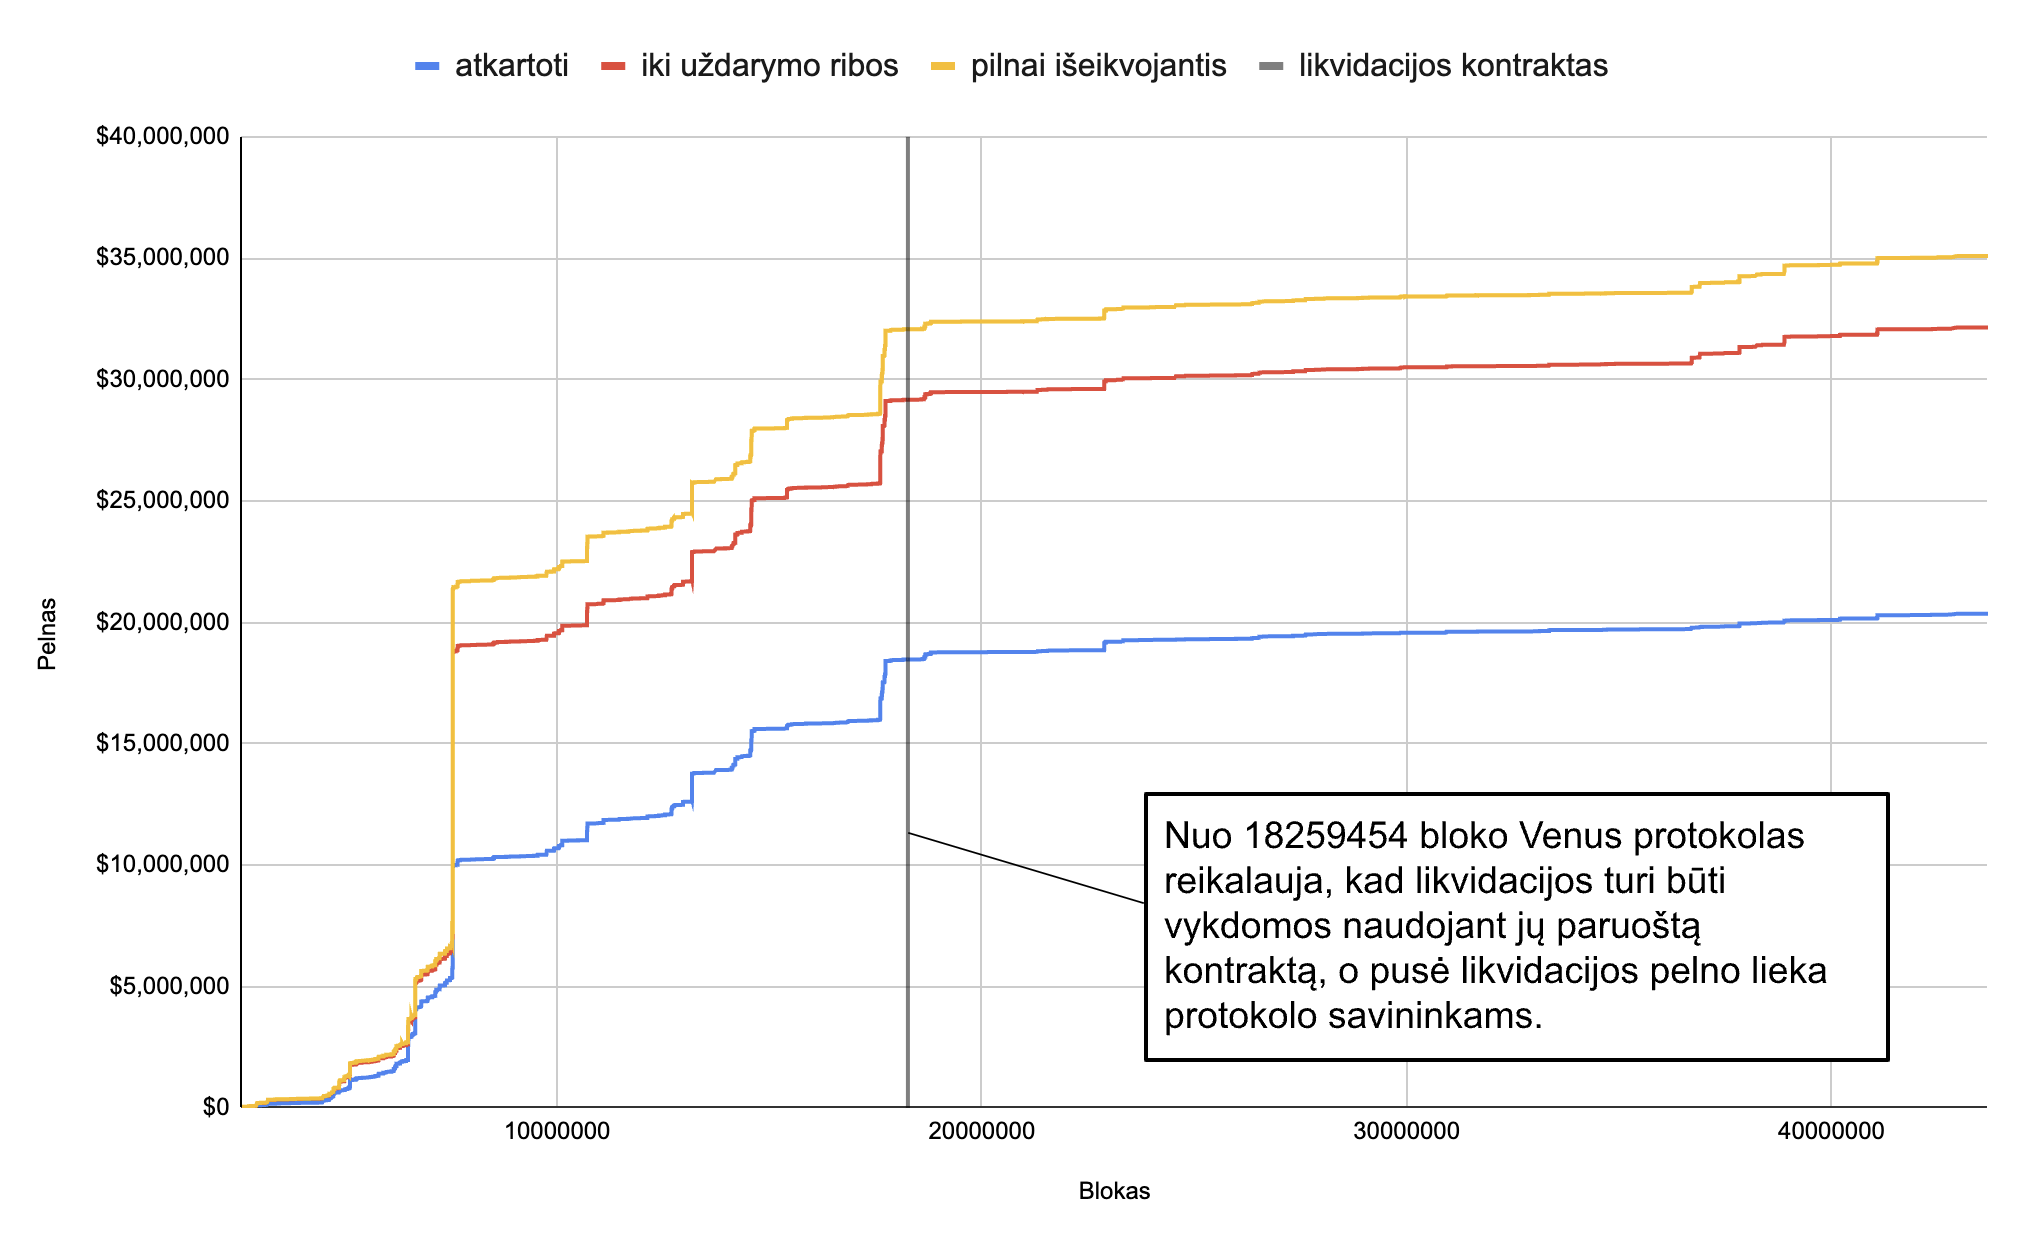
\includegraphics[scale=0.3]{resources/bendras4.png}
        \caption{Kaupiamasis pelnas pagal strategijas, atsižvelgiant tik į pirmąją kiekvieno skolininko likvidaciją}
        \label{img:bendras2}
      \end{figure}
\end{frame}

\section{Rezultatai}
\begin{frame}{Pagrindiniai rezultatai}
    \begin{table}[h!]
        \centering
        \label{tab:strategiju_pelnai}
        \begin{tabular}{|l|r|}
        \hline
        \textbf{Strategija}                     & \textbf{Pelnas (\$)} \\ \hline
        Atkartoti                               & 20 355 860,62        \\ \hline
        Iki uždarymo ribos              & 32 149 135,99        \\ \hline
        Pilnas išeikvojimas                           & 35 089 532,28        \\ \hline
        \end{tabular}
        \caption{Strategijų pelnai, atsižvelgiant tik į
        pirmąją kiekvieno skolininko likvidaciją}
    \end{table}
    \begin{itemize}
%Istoriniai duomenys atskleidė, kad ne visi likvidatoriai maksimaliai išnaudojo leidžiamą likvidacijos potencialą. Iki uždarymo ribos strategija, nors ir paprasta, generavo 58\% didesnį pelną lyginant su istorinių likvidacijų rezultatais 
    \item Daugelis likviduoja mažiau, nei leidžia protokolas. 
        \begin{itemize}
        \item \(\Rightarrow\) dėl to prarandama iki 58\% potencialaus pelno.
        \end{itemize}
    \item Naudojant pasiūlytą strategiją \emph{„Pilnas išeikvojimas“}, galima papildomai gauti iki 9\% daugiau pelno, lyginant su \emph{„Iki uždarymo ribos“}.
    \item Kai kuriais atvejais, kai skolininkas yra itin daug įsiskolinęs, \emph{„Pilno išeikvojimo“} strategija leidžia padvigubinti pelną.
    \end{itemize}
\end{frame}

\section{Išvados ir rekomendacijos}
\begin{frame}{Išvados}
  \begin{itemize}
    \item \textit{Pilnas išeikvojimas}, nors ir reikalauja daugiau likvidacijos iškvietimų, gali dar labiau padidinti pelną.
    % \item Likvidavimo algoritmo optimizavimas gali ženkliai padidinti likvidatorių pelną, bet kartu didėja ir „gas“ sąnaudos, bei reikalauja sudetingesnės logikos realizacijos.
    % \item Didžiausi pelno šuoliai pastebimi nedaugelyje stambių pozicijų likvidacijų.
    \item Reikšminga dalis papildomo pelno atsiranda iš palyginti nedidelio skaičiaus įvykių, kurie gali būti atsitiktiniai ir nebūtinai reprezentatyvūs būsimoms likvidacijoms.
  \end{itemize}
\end{frame}

\begin{frame}
  \centering
  \Large Klausimai?
\end{frame}

\end{document}
